\documentclass[12pt,oneside,a4paper,english]{article}
\usepackage[T1]{fontenc}
\usepackage[utf8]{inputenc}
\usepackage[margin=2.25cm,headheight=26pt,includeheadfoot]{geometry}
\usepackage[english]{babel}
\usepackage{listings}
\usepackage[table,xcdraw]{xcolor}
\usepackage{titlesec}
\usepackage{titling}
\usepackage[framed, numbered]{matlab-prettifier}
\usepackage{changepage}
\usepackage{changepage}
\usepackage{textgreek}
\usepackage{amsmath}
\usepackage{hyperref}
\hypersetup{hidelinks}
\usepackage{enumitem}
\usepackage{graphicx}
\usepackage{fancyhdr}
\usepackage{lastpage}
\usepackage{caption}
\usepackage{tocloft}
\usepackage{setspace}
\usepackage{multirow}
\usepackage{titling}
\usepackage{float}
\usepackage{comment}
\usepackage{booktabs}
\usepackage{indentfirst}
\usepackage{lscape}
\usepackage{booktabs,caption}
\usepackage[flushleft]{threeparttable}
\usepackage[english]{nomencl}
\makenomenclature
\usepackage{xcolor}
\usepackage{lipsum}
\usepackage{tabularx}
\usepackage{subcaption}
\usepackage{courier}
\usepackage{listings}
\usepackage{amsmath}
\usepackage{amssymb}


%%%%%%%
\usepackage{siunitx} % For alignment and formatting of numbers % I ADD THIS
\renewcommand{\thesubsection}{\thesection.\alph{subsection}}

%%%%%%
% --- set footer and header ---
\pagestyle{fancy}
\fancyhf{}

\setlength{\parindent}{2em}
\title{Assignment 1} % to reference as \title, dont use \maketitle
\makeatletter\let\Title\@title\makeatother



\lstset{language=Matlab,
style=Matlab-editor,
basicstyle=\normalsize\mlttfamily,
numbers=left,
numberstyle={\scriptsize\color{black}},			% size of the numbers
numbersep=0.5cm											
}

\newlist{steps}{enumerate}{1}
\setlist[steps, 1]{leftmargin=1.5cm,label = Step \arabic*:}
\renewcommand{\headrulewidth}{1pt}
\renewcommand{\footrulewidth}{1pt}

%\lhead{\Title}
\rhead{\nouppercase{\rightmark}}
\lhead{\Title}
\rfoot{
\includegraphics[height=1.25cm]{root/logo.pdf}} % right header logo
\setlength\headheight{16pt}
\setlength{\footskip}{50pt}
\lhead{\Title} %rightH title
\cfoot{\thepage}

% --- End of page settings ---



\begin{document}
\pagenumbering{roman} 

\begin{titlepage}
\begin{center}
\vspace{2cm}
%\textsc{ Danmarks Tekniske Universitet}\\[1.5cm]

\includegraphics[width=0.4\textwidth]{root/logo.pdf}~\\[1cm]
\vspace{2cm}


% Title
\hrule
\vspace{.5cm}
{\huge\bfseries
\begin{spacing}{1.05}
Multicore Semantics and Programming - Assignment 2
\end{spacing}
}
\vspace{.5cm}


\hrule
\vspace{1.5cm}

\textsc{\textbf{Author}}\\
\vspace{.5cm}
\centering

% add your name here
Kyle Fram - kdf25\\

\vspace{3cm}

\textsc{\textbf{Lecturers}}\\
\vspace{.5cm}
\centering

% add your name here
Professors Tim Harris and Peter Sewell\\

\vspace{1cm}



\centering \today % Dags dato
\end{center}
\end{titlepage}

\newpage
\doublespacing

\newpage
%\addcontentsline{toc}{section}{Table of Contents}
\renewcommand{\baselinestretch}{1}\normalsize
\tableofcontents
\renewcommand{\baselinestretch}{1}\normalsize
%\singlespacing
\thispagestyle{fancy} % force page style

% Add the list of abbreviations here
% \newpage
% \printnomenclature
% \addcontentsline{toc}{section}{Nomenclature}

\newpage
\pagenumbering{arabic} 
\fancyfoot[C]{Page \thepage\ of \pageref{EndOfText}}


% part 1
I have written the estimated time for each part in parentheses under subsection label. Generally, setting up diy and opam, as well as relearning a bit of C, made up the lion's share of the time.

\section{} \label{}
% details on diy7 etc 
%https://diy.inria.fr/doc/gen.html#diycross%3Aintro 
\subsection{(2 hours)}
We use these commands to generate the tests:
\begin{lstlisting}
    diyone7 -arch AArch64 "PodWR Fre PodWR Fre" -name SB
    diyone7 -arch AArch64 "PodWR Fre PodWR Fre PodWR Fre" -name SB3    
    diyone7 -arch AArch64 "DMB.SYdWR Fre DMB.SYdWR Fre" -name SB+fen 
    diyone7 -arch AArch64 "DMB.SYdWR Fre DMB.SYdWR Fre DMB.SYdWR Fre" -name SB3+fen
\end{lstlisting}

'SB3' is my shorthand for Store Buffering with 3 threads. 
I am on an M4 Max chip (AArch64), and I expect to observe significant relaxations in the unfenced SB and SB3 tests.

\lstinputlisting[caption={System Specs}, label={lst:specs}]{../logs/q1/sys_summary.txt}

\subsection{(30 min)}

Running with litmus7, we notice 7.7 and 9.4 seconds to run SB with and without barrier respectively. 
As expecteed, the test condition is not validated in the fenced case, but is in the unfenced case.

For SB3, we see 10.4 and 12.4 seconds respectively, a slightly higher percentage difference (81\% vs 83\%). 
We see the expected fenced vs unfenced results. 

Another curious difference is that while unfenced SB has only 234 out of 1e8 iterations validating the test condition, SB3 has 1870409 out of 1e8 iterations validating the test condition.
We may see more prevalent compiler optimization and reordering in the latter case with more threads, 
possibly the extra thread results in more optimization opportunities.

Using -s 1k, -r 100k to get 1e8 for each case:

\begin{lstlisting}
    litmus7 SB.litmus -s 1k -r 100k > logs/q1/b_1.txt 
    litmus7 SB+fen.litmus -s 1k -r 100k > logs/q1/b_1fen.txt     
    litmus7 SB3.litmus -s 1k -r 100k > logs/q1/b_2.txt 
    litmus7 SB3+fen.litmus -s 1k -r 100k > logs/q1/b_2fen.txt 
\end{lstlisting}


\subsection{(2 min)}

Comparing the axiomatic results, we naturally notice no difference in timing. 
However we notice the expected difference in the results, with our test condition missing from possible outputs in the fenced cases. 

\begin{lstlisting}
    herd7 SB.litmus > logs/q1/c_1.txt 
    herd7 SB3.litmus > logs/q1/c_1fen.txt  
    herd7 SB+fen.litmus > logs/q1/c_2.txt
    herd7 SB3+fen.litmus > logs/q1/c_2fen.txt
\end{lstlisting}
%https://www.cl.cam.ac.uk/~sf502/regressions/rmem/help.html

\subsection{(30 min)}
We use interactive -false and eager -true flags. 
In both cases, the fenced version notes 'allowed not found'  agreeing with prior analaysis. 
\begin{lstlisting}    
    rmem -model flat -interactive false -eager true SB.litmus > logs/q1/d_1.txt
    rmem -model flat -interactive false -eager true SB+fen.litmus > logs/q1/d_1fen.txt
    rmem -model flat -interactive false -eager true SB3.litmus > logs/q1/d_2.txt      
    rmem -model flat -interactive false -eager true SB3+fen.litmus > logs/q1/d_2fen.txt
\end{lstlisting}

\subsection{(20 min)}
Again, we reinforced the expected results from the above. 
\begin{lstlisting}
    mcompare7 logs/q1/b_1.txt logs/q1/c_1.txt > logs/q1/e_1.txt
    mcompare7 logs/q1/b_1fen.txt logs/q1/c_1fen.txt > logs/q1/e_1fen.txt
    mcompare7 logs/q1/b_2.txt logs/q1/c_2.txt > logs/q1/e_2.txt
    mcompare7 logs/q1/b_2fen.txt logs/q1/c_2fen.txt > logs/q1/e_2fen.txt
    
\end{lstlisting}


%LINK: 
% https://www.cl.cam.ac.uk/~sf502/regressions/rmem/

\newpage
\section{}
\subsection{(45 min)}
Forbidden by ARM ARM. 
Consider \href{https://developer.arm.com/documentation/ddi0487/maa/-Part-B-The-AArch64-Application-Level-Architecture/-Chapter-B2-The-AArch64-Application-Level-Memory-Model/-B2-3-Ordering-requirements-defined-by-the-formal-concurrency-model/-B2-3-2-Intrinsic-Dependency-relations?lang=en}{B.2.3.2}. 
The important note here is in the Note box: 
"This applies even in cases where the Intrinsic Data Dependency might be perceived to be a false dependency." 
Further, this is a 'data dependency' as defined by \href{https://developer.arm.com/documentation/ddi0487/maa/-Part-B-The-AArch64-Application-Level-Architecture/-Chapter-B2-The-AArch64-Application-Level-Memory-Model/-B2-3-Ordering-requirements-defined-by-the-formal-concurrency-model/-B2-3-6-Dependency-relations?lang=en}{B.2.3.6},  
and since this architecture respects data dependencies and coherence, the memory accesses must follow in strict order, and therefore $x=3$ is forbidden. 

\subsection{(10 min)}
RISC-V as per \href{https://docs.riscv.org/reference/isa/unpriv/rvwmo.html#17-1-1-3-preserved-program-order}{17.1.1.3}, rule 10 enforces PPO over data dependencies, 
such that the $d:y=1$ read and corresponding $e:x=1$ write must be ordered after the $x=3$ write, and thus according to the 
\href{https://docs.riscv.org/reference/isa/unpriv/mm-eplan.html#preserved-program-order-and-global-memory-order}{Load Value Axiom}, 
would be 'latest' in global memory order and therefore $x=3$ must not be reachable in practice.


\subsection{(20 min)}

As per the above, on AArch64, the test is forbidden and we see axiomatically this is reinforced. 
We also ran 1e8 litmus tests and saw no positive witnesses, enforcing our result empirically. 

%    diyone7 -arch AArch64 "DMB.STdWW Rfe DMB.LDdRR Fre" -name S+fen+data-wsi 
\begin{lstlisting}
    diyone7 -arch AArch64 "Wse DMB.SYdWW Rfe DpDatadW" -name sub
    rmem -model flat -interactive false -eager true sub.litmus > logs/q2/c_1.txt
    herd7 sub.litmus > logs/q2/c.txt
\end{lstlisting}

\lstinputlisting{../logs/q2/c.txt}
\newpage
\section{}
\subsection{(45 min)}
% https://davekilian.com/acquire-release.html
Consider a 'fence' operation. This provides a 'synchronization point,' such that all memory operations before and after the fence wait for all others, and once all operations meet at the fence, they tear it down. 
Now, consider propping a ladder up on one side of the metaphorical fence. For an acquire or release, this synchronization is 'one-way,' so anyone on the far side cannot access until the last operation throws the ladder over the fence. 

\subsection{(3 hrs)}
I implemented Message Passing with pthreads and acquire/release semantics. 
This program has a writer thread which writes two values in succession with a release between the writes, 
and then a reader thread which reads those respectively with an acquire fence between them. 
Pthreads only allows one arg so I wrapped the values in a struct. 
The release/acquire semantics ensure that x=1,y=1 always holds at termination, but does not force the writer to wait for respective read. 

\lstinputlisting[caption={MessagePassing}, label={lst:MP}]{../ctests/raq.c}

\subsection{(5 min)}
In a certain sense, this is consistent, we have DMB ISH for the release and DMB ISHLD for the acquire. 
In another sense, this is redundant, as we are using atomics and the compiler uses stlr and ldar, which enforce sequential consistency anyhow. 
Overall this is indeed consistent, albeit redundant. \newline
Here is the compiled code (screenshots in appendix):

\lstinputlisting[caption={Compiled MessagePassing}, label={lst:MPC}]{../logs/q3/raq.txt}

\subsection{(10 min)}
Litmus test of the above:
\lstinputlisting[caption={MP with Release/Acquire Litmus}, label={lst:mpraq}]{../mpraq.litmus}

\subsection{(15 min)}
As above, we expect and see 'forbidden' here, we have this doubly redundant synchronization with fences and store-releases. 
\begin{lstlisting}
    cd ctests
    herd7 ../mpraq.litmus > ../logs/q3/e.txt
\end{lstlisting}
\lstinputlisting[caption={Litmus Results (herd7)}, label={lst:MPC}]{../logs/q3/e.txt}

\newpage
\section{}
\subsection{(2hr)}

We define $ppo$ to be the communication relation without the 'writes to the same location' relation as a relaxation of x86-TSO. 

\lstinputlisting{../cats/tsorel.cat}

\subsection{(20min)}

$S$ is a good test to verify our model due to its two writes to different memory locations. 
We expect different results in our relaxed model vs. the standard x86-TSO model.

\begin{lstlisting}
    
    diyone7 -arch AArch64 PodWW Rfe PodRW Wse -name S
    herd7 S.litmus -model cats/tsorel.cat>> logs/q4/b1.txt
    herd7 S.litmus > logs/q4/b2.txt 

\end{lstlisting}

Indeed we see that in the relaxed model, we sometimes see the 'reordered' outcome, where in TSO we never see this. 

\lstinputlisting[caption={Litmus Results (herd7) (PPO Model)}, label={lst:tsorel}]{../logs/q4/b1.txt}
\lstinputlisting[caption={Litmus Results (herd7) (x86 TSO Model)}, label={lst:tsorel}]{../logs/q4/b2.txt}

\subsection{(30 min)}
Here is the paper math definition of the relaxed model based on the x86-tso model referenced in \cite{alglave2014herding}:

Starting from the definitions in the notes and slides:


\begin{flalign*}
E &= \{e \mid e \in \{e_1, \dots, e_n\} \land (\text{iswrite}(e) \lor \text{isread}(e))\} & \\
\text{po} &= \{(e, e') \mid e \in E \land e' \in E \land e < e' \land \text{thread}(e) = \text{thread}(e')\} & \\
\text{wr} &= \text{po} \land (\text{iswrite}(e) \land \text{isread}(e')) & \\
\text{ww} &= \text{po} \land \text{iswrite}(e) \land \text{iswrite}(e') \land (\text{addr}(e) \neq \text{addr}(e')) & \\
\text{ppo} &= \text{po} \setminus (\text{ww} \lor \text{wr}) & \\
\text{acyclic}& (\text{ppo} \mid \text{com}) \text{as } \text{sc} &
\end{flalign*}


\subsection{(1 min)}

C allows for this sort of relaxation natively with stdatomic and memory\_order\_relaxed.
If these are executed with memory\_order\_relaxed on ARM for example, two writes to different locations may be reordered. 

\subsection{(5 min)}

Arbitrarily reordering of reads from different locations may be more tricky. 
Take Message Passing for example, arbitrary reordering of reads of different locations effectively 
breaks any notion of intrathread communication, and fencing, reliance on atomicity, or at least acquire/release must be used often. 
Realistically, a language without fences, barriers, or sequential reads becomes chaos. 
\newpage

\setcounter{section}{0}

\section{Appendix}
\subsection{diy7}
\subsection{litmus7}
\lstinputlisting[caption={SB.litmus}, label={lst:SB}]{../logs/q1/b_1.txt}
\lstinputlisting[caption={SB.litmus}, label={lst:SB}]{../logs/q1/b_1fen.txt}    
\lstinputlisting[caption={SB3.litmus}, label={lst:SB3}]{../logs/q1/b_2.txt}
\lstinputlisting[caption={SB3.litmus}, label={lst:SB3}]{../logs/q1/b_2fen.txt}
\subsection{herd7}
\lstinputlisting[caption={SB.litmus}, label={lst:SB}]{../logs/q1/c_1.txt}
\lstinputlisting[caption={SB.litmus}, label={lst:SB}]{../logs/q1/c_1fen.txt}    
\lstinputlisting[caption={SB3.litmus}, label={lst:SB3}]{../logs/q1/c_2.txt}
\lstinputlisting[caption={SB3.litmus}, label={lst:SB3}]{../logs/q1/c_2fen.txt}
\subsection{rmem}
\lstinputlisting[caption={SB.litmus}, label={lst:SB}]{../logs/q1/d_1.txt}
\lstinputlisting[caption={SB.litmus}, label={lst:SB}]{../logs/q1/d_1fen.txt}    
\lstinputlisting[caption={SB3.litmus}, label={lst:SB3}]{../logs/q1/d_2.txt}
\lstinputlisting[caption={SB3.litmus}, label={lst:SB3}]{../logs/q1/d_2fen.txt}
\subsection{mcompare7}
\lstinputlisting[caption={SB.litmus}, label={lst:SB}]{../logs/q1/e_1.txt}
\lstinputlisting[caption={SB.litmus}, label={lst:SB}]{../logs/q1/e_1fen.txt}    
\lstinputlisting[caption={SB3.litmus}, label={lst:SB3}]{../logs/q1/e_2.txt}
\lstinputlisting[caption={SB3.litmus}, label={lst:SB3}]{../logs/q1/e_2fen.txt}

\newpage
\section{Appendix}

\subsection{}
\lstinputlisting[caption={sub.litmus}, label={lst:sub}]{../logs/q2/c.txt}
%\lstinputlisting[caption={sub.litmus}, label={lst:sub}]{../logs/q2/c_2.txt}

\newpage
\section{Appendix}
 \_\newline
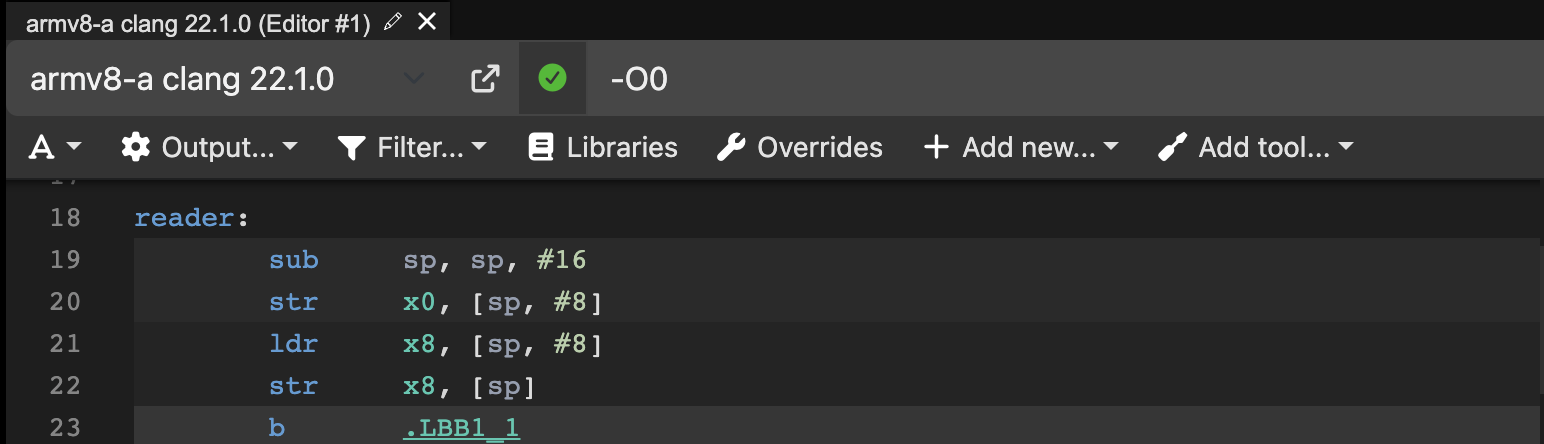
\includegraphics[width=\textwidth]{../logs/q3/images/reader.png}
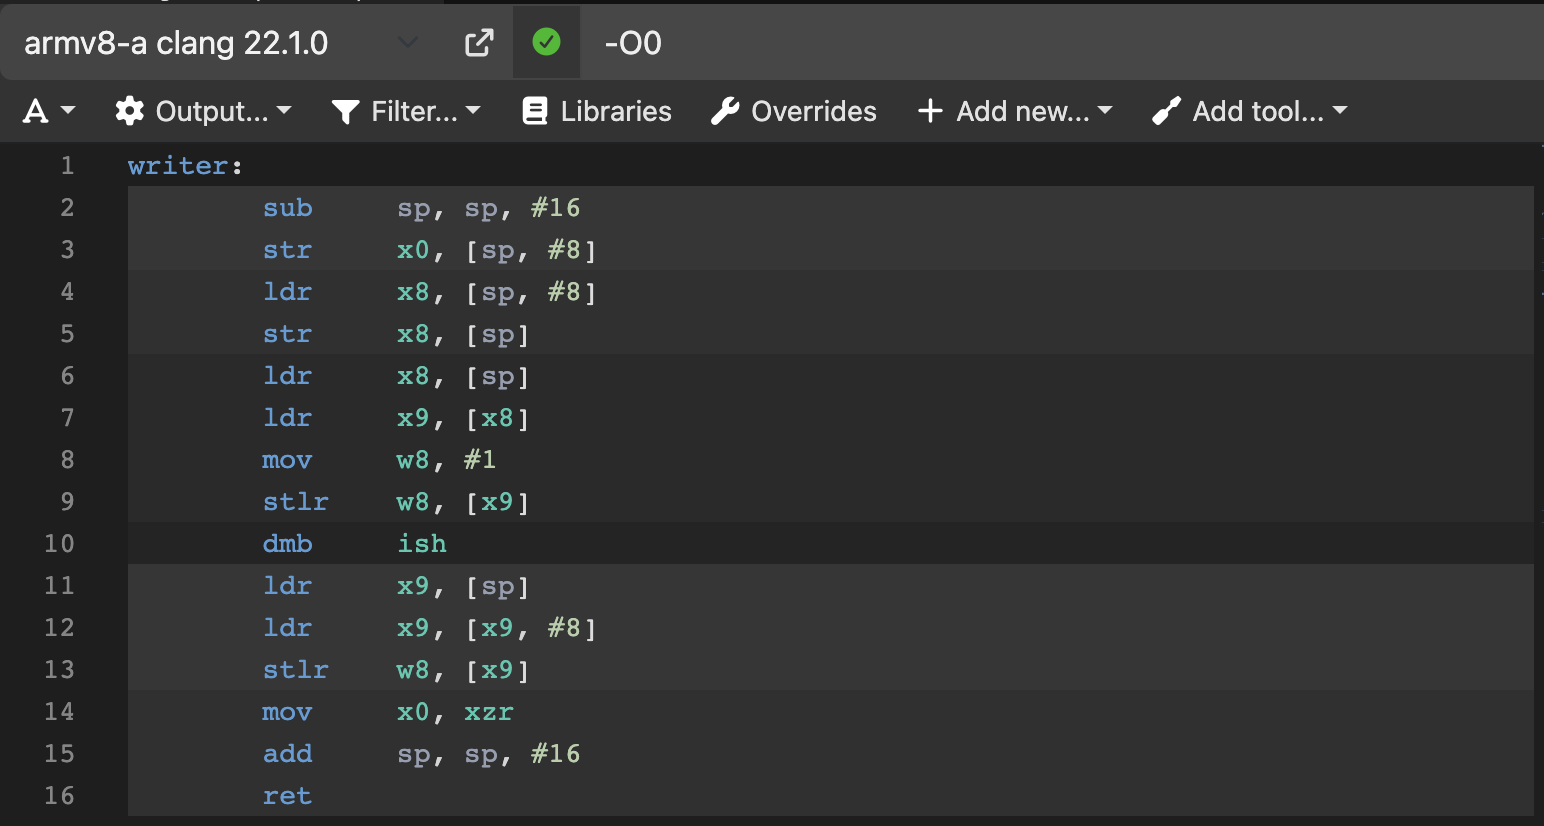
\includegraphics[width=\textwidth]{../logs/q3/images/writer.png}
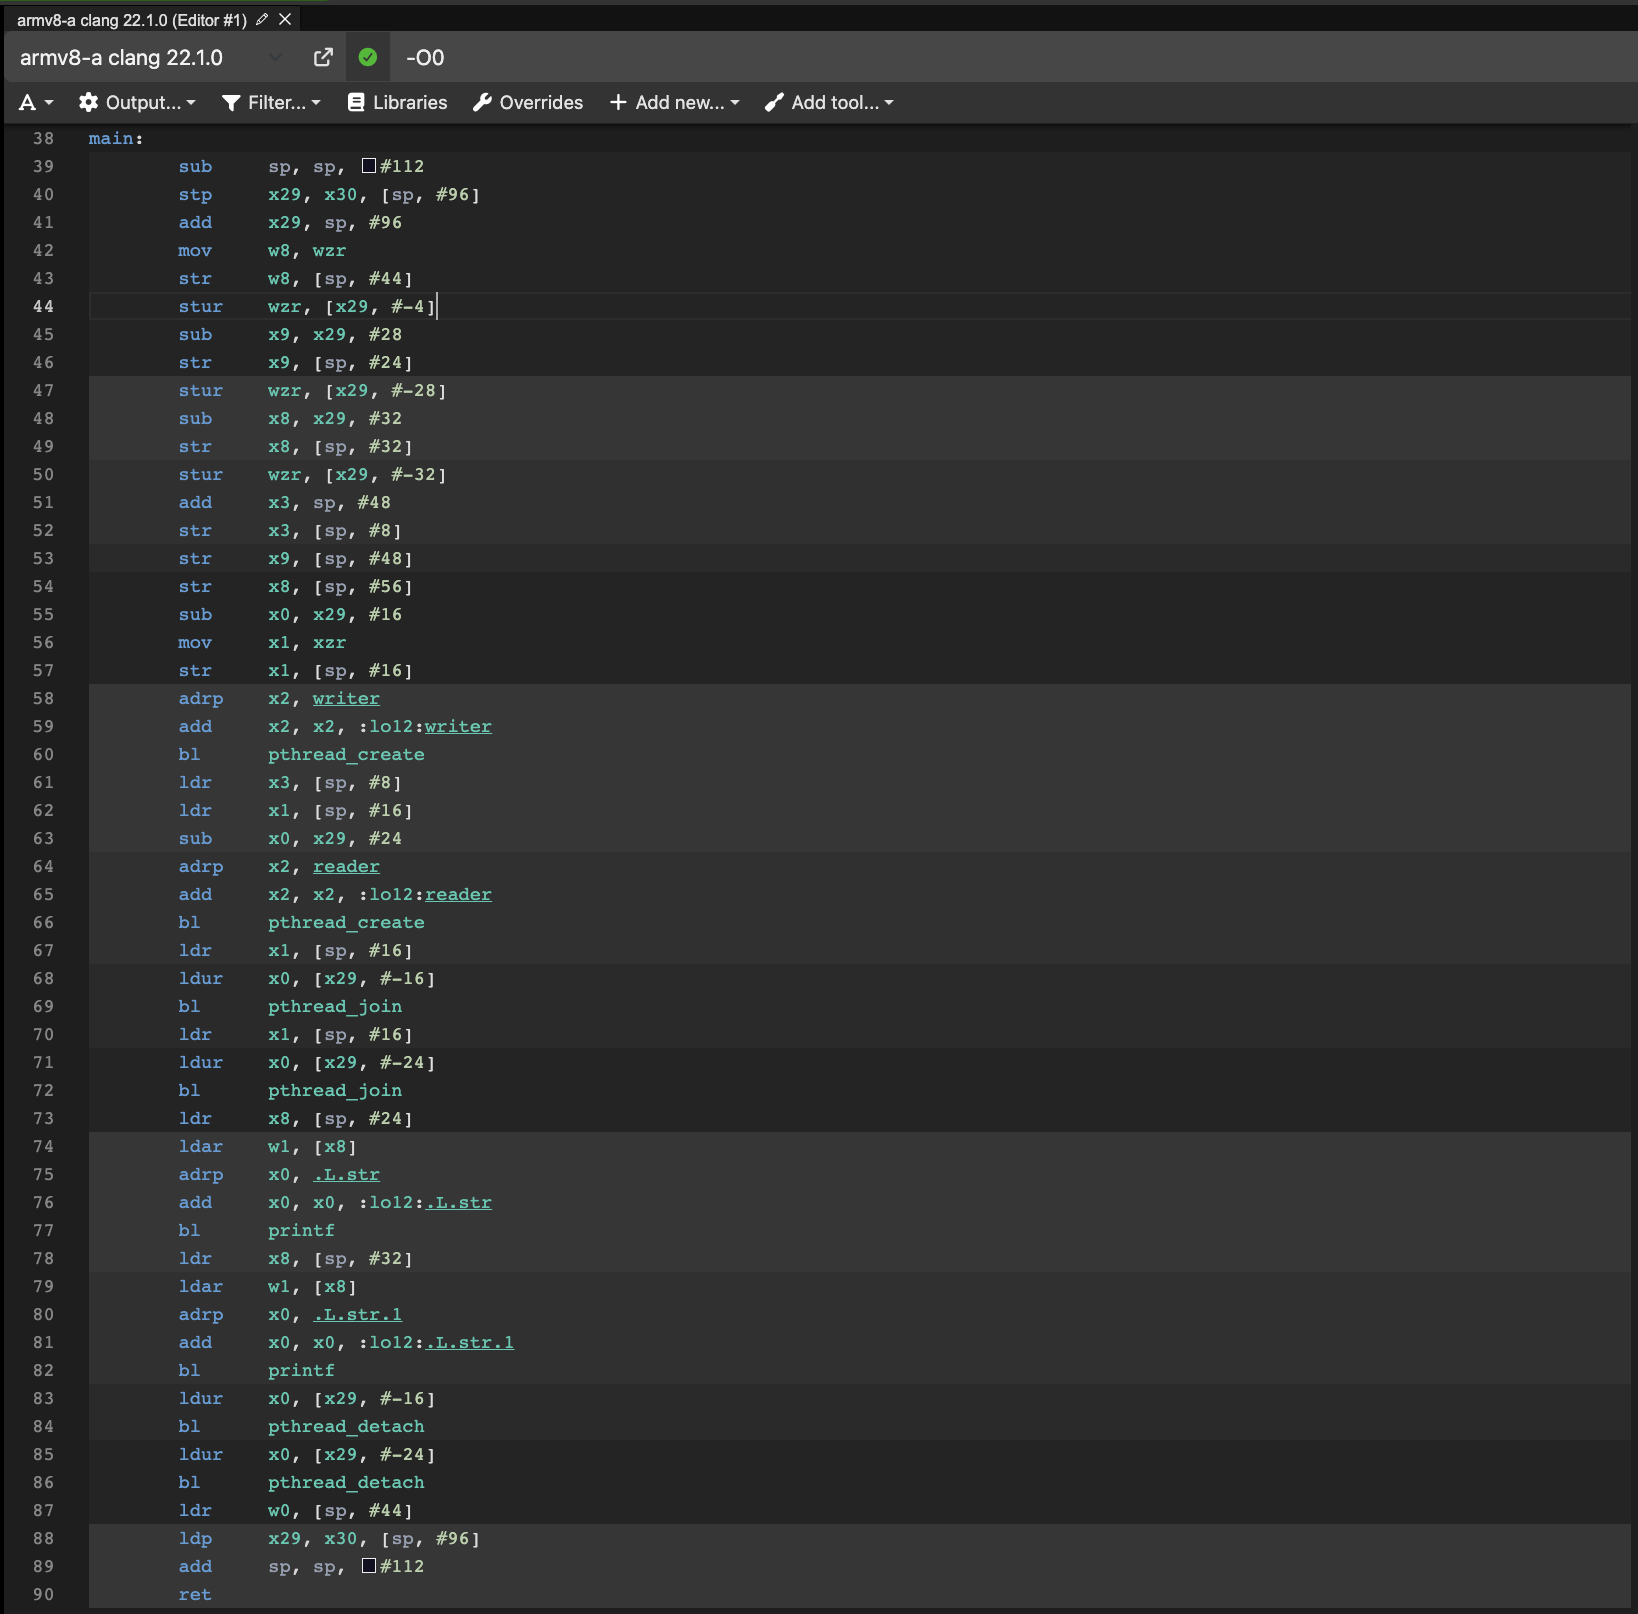
\includegraphics[width=\textwidth]{../logs/q3/images/main.png}



\newpage
\addcontentsline{toc}{section}{References}
\fancyfoot[C]{Page \thepage\ of \pageref{endOfDoc}}
\nocite{*}
\bibliography{document.bib} 
\bibliographystyle{ieeetr}

\input{}


\label{EndOfText}

\newpage
\pagenumbering{Roman} 
\addcontentsline{toc}{section}{List of Figures}
\fancyfoot[C]{Page \thepage\ of \pageref{endOfDoc}}
\listoffigures
\thispagestyle{fancy}

\newpage
\addcontentsline{toc}{section}{List of Tables}
\listoftables
\thispagestyle{fancy}

\label{endOfDoc}
\end{document}
